% GauCon Architecture Figure (English WACV 2-column exact width: ~495 pt, zero node overlap)
% Matches src/tinydet/modules/lgt_detect.py and src/tinydet/models/ultralytics.py (ac79514).
\documentclass[tikz,border=2pt]{standalone}
\usepackage{fontspec}
\usepackage{amsmath,amssymb}
\setmainfont{DejaVu Serif}
\usetikzlibrary{positioning,fit,calc,arrows.meta,backgrounds}

% Okabe-Ito harmonized academic palette
\definecolor{cIn}{HTML}{EDF2F7}
\definecolor{cBack}{HTML}{D6EAF8}
\definecolor{cGauCon}{HTML}{FDEBD0}
\definecolor{cId}{HTML}{E8F8F5}
\definecolor{cTrain}{HTML}{F5EEF8}
\definecolor{cBox}{HTML}{FADBD8}
\definecolor{cCls}{HTML}{D4EFDF}
\definecolor{cEdge}{HTML}{1F2937}
\definecolor{cTrainEdge}{HTML}{6C3483}

\begin{document}
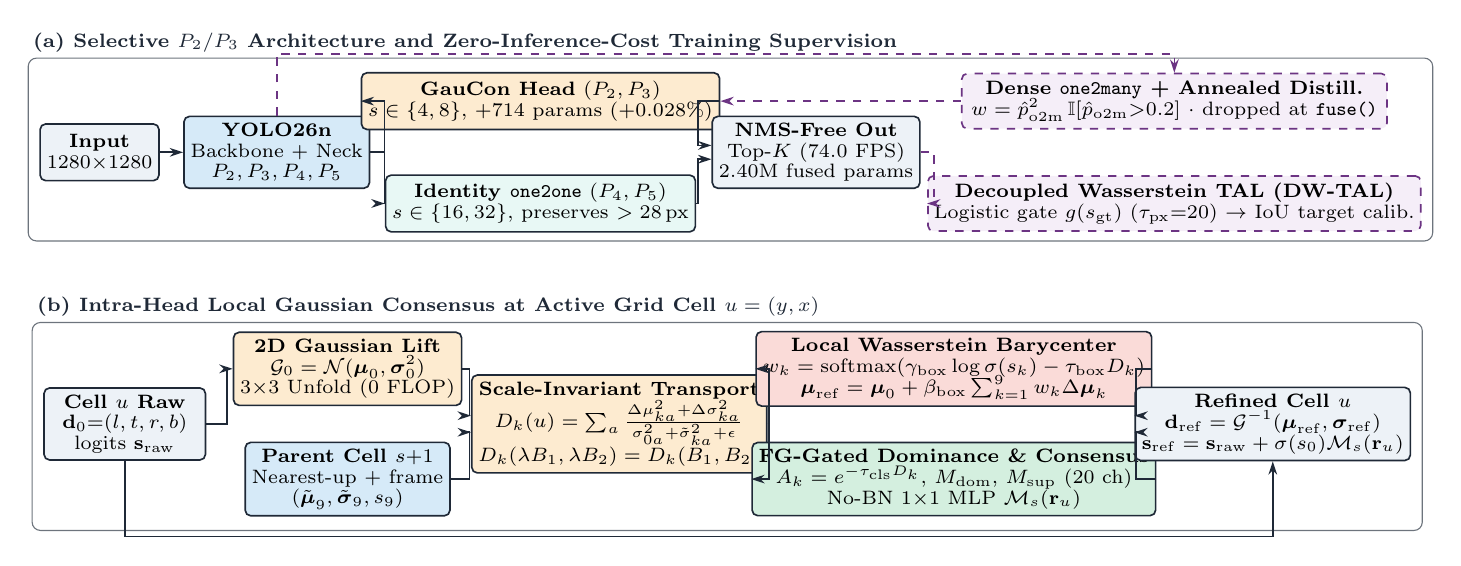
\begin{tikzpicture}[
  x=1cm, y=1cm,
  font=\scriptsize,
  blk/.style={draw=cEdge, fill=#1, semithick, rounded corners=2pt,
              align=center, inner sep=2.4pt, minimum height=7.2mm},
  tblk/.style={draw=cTrainEdge, dashed, fill=#1, semithick, rounded corners=2pt,
               align=center, inner sep=2.2pt, minimum height=7.0mm},
  arr/.style={-{Stealth[length=1.7mm,width=1.1mm]}, cEdge, semithick},
  tarr/.style={-{Stealth[length=1.7mm,width=1.1mm]}, cTrainEdge, dashed, semithick},
  grp/.style={draw=cEdge!65, rounded corners=3pt, inner sep=4pt},
  ptitle/.style={font=\scriptsize\bfseries, text=cEdge, fill=white, inner sep=1.8pt},
]

% =========================================================================
% PANEL (a): Selective P2/P3 GauCon Pipeline & Zero-Cost Training Supervision
% Total width span: x in [0.0, 17.2] cm (~492 pt = 0.994 \textwidth)
% =========================================================================
\node[blk=cIn, minimum width=1.40cm] (img) at (0.70, 5.20) {\textbf{Input}\\[-0.5pt]$1280{\times}1280$};

\node[blk=cBack, minimum width=2.20cm] (fpn) at (2.95, 5.20) {\textbf{YOLO26n}\\[-0.5pt]Backbone + Neck\\[-0.5pt]$P_2, P_3, P_4, P_5$};

\node[blk=cGauCon, minimum width=3.35cm] (p23) at (6.30, 5.85) {\textbf{GauCon Head} ($P_2, P_3$)\\[-0.5pt]$s\in\{4,8\}$, $+714$ params ($+0.028\%$)};

\node[blk=cId, minimum width=3.35cm] (p45) at (6.30, 4.55) {\textbf{Identity \texttt{one2one}} ($P_4, P_5$)\\[-0.5pt]$s\in\{16,32\}$, preserves $>28$\,px};

\node[blk=cIn, minimum width=2.35cm] (out) at (9.80, 5.20) {\textbf{NMS-Free Out}\\[-0.5pt]Top-$K$ ($74.0$ FPS)\\[-0.5pt]$2.40$M fused params};

\node[tblk=cTrain, minimum width=5.40cm] (o2m) at (14.35, 5.85) {\textbf{Dense \texttt{one2many} + Annealed Distill.}\\[-0.5pt]$w = \hat{p}_{\mathrm{o2m}}^2\,\mathbb{I}[\hat{p}_{\mathrm{o2m}}{>}0.2]$ $\cdot$ dropped at \texttt{fuse()}};

\node[tblk=cTrain, minimum width=5.40cm] (dwtal) at (14.35, 4.55) {\textbf{Decoupled Wasserstein TAL (DW-TAL)}\\[-0.5pt]Logistic gate $g(s_{\mathrm{gt}})$ ($\tau_{\mathrm{px}}{=}20$) $\to$ IoU target calib.};

\draw[arr] (img.east) -- (fpn.west);
\draw[arr] (fpn.east) -- (4.32, 5.20) |- (p23.west);
\draw[arr] (fpn.east) -- (4.32, 5.20) |- (p45.west);
\draw[arr] (p23.east) -- (8.30, 5.85) |- ([yshift=2.5pt]out.west);
\draw[arr] (p45.east) -- (8.30, 4.55) |- ([yshift=-2.5pt]out.west);

\draw[tarr] (fpn.north) -- (2.95, 6.45) -- (14.35, 6.45) -- (o2m.north);
\draw[tarr] (o2m.west) -- (p23.east);
\draw[tarr] (out.east) -- (11.30, 5.20) |- (dwtal.west);

\begin{scope}[on background layer]
  \node[grp, fit=(img)(fpn)(p23)(p45)(out)(o2m)(dwtal), yshift=1pt,
        label={[ptitle, anchor=south west]north west:{(a) Selective $P_2/P_3$ Architecture and Zero-Inference-Cost Training Supervision}}] {};
\end{scope}

% =========================================================================
% PANEL (b): Intra-Head Local Gaussian Consensus at Active Cell u = (y, x)
% =========================================================================
\node[blk=cIn, minimum width=2.05cm] (raw) at (1.02, 1.75) {\textbf{Cell $u$ Raw}\\[-0.5pt]$\mathbf{d}_0{=}(l,t,r,b)$\\[-0.5pt]logits $\mathbf{s}_{\mathrm{raw}}$};

\node[blk=cGauCon, minimum width=2.45cm] (lift) at (3.85, 2.45) {\textbf{2D Gaussian Lift}\\[-0.5pt]$\mathcal{G}_0 = \mathcal{N}(\boldsymbol{\mu}_0, \boldsymbol{\sigma}_0^2)$\\[-0.5pt]$3{\times}3$ Unfold ($0$ FLOP)};

\node[blk=cBack, minimum width=2.45cm] (par) at (3.85, 1.05) {\textbf{Parent Cell $s{+}1$}\\[-0.5pt]Nearest-up + frame\\[-0.5pt]$(\tilde{\boldsymbol{\mu}}_9, \tilde{\boldsymbol{\sigma}}_9, s_9)$};

\node[blk=cGauCon, minimum width=3.15cm] (dist) at (7.30, 1.75) {\textbf{Scale-Invariant Transport}\\[-0.5pt]$D_k(u) = \sum_{a}\frac{\Delta\mu_{ka}^2 + \Delta\sigma_{ka}^2}{\sigma_{0a}^2 + \tilde{\sigma}_{ka}^2 + \epsilon}$\\[-0.5pt]$D_k(\lambda B_1,\lambda B_2) = D_k(B_1,B_2)$};

\node[blk=cBox, minimum width=4.05cm] (bary) at (11.55, 2.45) {\textbf{Local Wasserstein Barycenter}\\[-0.5pt]$w_k = \mathrm{softmax}(\gamma_{\mathrm{box}}\log\sigma(s_k) - \tau_{\mathrm{box}}D_k)$\\[-0.5pt]$\boldsymbol{\mu}_{\mathrm{ref}} = \boldsymbol{\mu}_0 + \beta_{\mathrm{box}}\sum_{k=1}^9 w_k\Delta\boldsymbol{\mu}_k$};

\node[blk=cCls, minimum width=4.05cm] (gate) at (11.55, 1.05) {\textbf{FG-Gated Dominance \& Consensus}\\[-0.5pt]$A_k = e^{-\tau_{\mathrm{cls}}D_k}$, $M_{\mathrm{dom}}$, $M_{\mathrm{sup}}$ ($20$ ch)\\[-0.5pt]No-BN $1{\times}1$ MLP $\mathcal{M}_s(\mathbf{r}_u)$};

\node[blk=cIn, minimum width=2.90cm] (refout) at (15.60, 1.75) {\textbf{Refined Cell $u$}\\[-0.5pt]$\mathbf{d}_{\mathrm{ref}} = \mathcal{G}^{-1}(\boldsymbol{\mu}_{\mathrm{ref}}, \boldsymbol{\sigma}_{\mathrm{ref}})$\\[-0.5pt]$\mathbf{s}_{\mathrm{ref}} = \mathbf{s}_{\mathrm{raw}} + \sigma(s_0)\mathcal{M}_s(\mathbf{r}_u)$};

\draw[arr] (raw.east) -- (2.32, 1.75) |- (lift.west);
\draw[arr] (raw.south) -- (1.02, 0.32) -- (15.60, 0.32) -- (refout.south);
\draw[arr] (lift.east) -- (5.40, 2.45) |- ([yshift=3pt]dist.west);
\draw[arr] (par.east) -- (5.40, 1.05) |- ([yshift=-3pt]dist.west);
\draw[arr] (dist.east) -- (9.20, 1.75) |- (bary.west);
\draw[arr] (dist.east) -- (9.20, 1.75) |- (gate.west);
\draw[arr] (bary.east) -- (13.86, 2.45) |- ([yshift=3pt]refout.west);
\draw[arr] (gate.east) -- (13.86, 1.05) |- ([yshift=-3pt]refout.west);

\begin{scope}[on background layer]
  \node[grp, fit=(raw)(lift)(par)(dist)(bary)(gate)(refout), yshift=-1pt,
        label={[ptitle, anchor=south west]north west:{(b) Intra-Head Local Gaussian Consensus at Active Grid Cell $u = (y, x)$}}] {};
\end{scope}

\end{tikzpicture}
\end{document}
